\documentclass[conference]{IEEEtran}
\IEEEoverridecommandlockouts

\usepackage{cite}
\usepackage[numbers]{natbib}
\usepackage{amsmath,amssymb,amsfonts}
\usepackage{algorithm}
\usepackage{algpseudocode}
\usepackage{xcolor}
\usepackage{graphicx}
\usepackage[warn]{textcomp}
\usepackage{multirow}
\usepackage{mathtools}
\usepackage{commath}
\usepackage{caption}
\usepackage{subcaption}
\usepackage[super]{nth}
\usepackage{url}
\usepackage{tabularx}
\usepackage{longtable,multicol,makecell}
\usepackage{pgfplots}


\def\UrlBreaks{\do\/\do-}

% tikz
\usepackage{tikz}
\usetikzlibrary{shapes.geometric, arrows}
% tikz styles
\tikzstyle{user} = [circle, thick, draw, minimum size=2.5cm]
\tikzstyle{item} = [rectangle, thick, draw, minimum width=3cm, minimum height=1.5cm]
\tikzstyle{arrow} = [->, draw, thick]
\tikzstyle{bi-arrow} = [<->, draw, thick]
\tikzstyle{line} = [-, draw, thick]

\def\BibTeX{{\rm B\kern-.05em{\sc i\kern-.025em b}\kern-.08em
    T\kern-.1667em\lower.7ex\hbox{E}\kern-.125emX}}

\emergencystretch=8em

\newcommand{\visresults}[2]{
    \begin{figure}[H]
        \centering
        \begin{subfigure}{.15\textwidth}
            \centering
            \includegraphics[width=1\linewidth]{images/results/#1/graph_#2.png}
            \caption{Graph}
        \end{subfigure}%
        %
        \begin{subfigure}{.15\textwidth}
            \centering
            \includegraphics[width=1\linewidth]{images/results/#1/embeddings_#2.png}
            \caption{Embeddings}
        \end{subfigure}%
        %
        \begin{subfigure}{.15\textwidth}
            \centering
            \includegraphics[width=1\linewidth]{images/results/#1/weights_#2.png}
            \caption{Weights}
        \end{subfigure}%
        %
        \caption{ComE with #1, $K=#2$}
        \label{fig:results#1#2}
    \end{figure}
}

\begin{document}

\title{Community Embeddings with Bayesian Gaussian Mixture Model and Variational Inference\\
    \thanks{The reported study was partially supported by RFBR grant \textnumero 20-07-00958. The paper was prepared within the framework of the HSE University Project Group Competition 2020-2022.}
}

\author{
    \IEEEauthorblockN{Anton I. N. Begehr}
    \IEEEauthorblockA{
        \textit{Graduate School of Business}\\
        \textit{National Research University Higher School of Economics}\\
        Moscow, Russia\\
        a.begehr@fu-berlin.de\\
    }
    \and
    \IEEEauthorblockN{Prof. Dr. Petr Panfilov}
    \IEEEauthorblockA{
        \textit{Graduate School of Business}\\
        \textit{National Research University Higher School of Economics}\\
        Moscow, Russia\\
        ppanfilov@hse.ru\\
    }
}

\maketitle

\begin{abstract}
    Graphs, such as social networks, emerge naturally from various real-world situations. Recently, graph embedding methods have gained traction in data science research.
    The graph and community embedding algorithm ComE aims to preserve first-, second- and higher-order proximity. ComE requires prior knowledge of the number of communities K. In this paper, ComE is extended to utilize a Bayesian Gaussian mixture model with variational inference for learning community embeddings (ComE BGMM+VI), similar to ComE+. ComE BGMM+VI takes K as the maximum number of communities and drops components through the trade-off hyperparameter weight concentration prior.
    The advantage of ComE BGMM+VI over the non-Bayesian ComE for an unknown number of communities K is shown for the small Karate club dataset and explored for the larger DBLP dataset.
\end{abstract}

\begin{IEEEkeywords}
    graph, embedding, community embedding, ComE, Bayesian, variational inference, Gaussian mixture, expectation maximization
\end{IEEEkeywords}


\section{Introduction}

Graphs, such as social networks, knowledge graphs, content-rating graphs, and communication networks, emerge naturally from various real-world situations. Analyzing these graphs leads to findings and understanding of the underlying structures, coherences, and dependencies. Recently, methods for embedding graph's nodes into lower-dimensional Euclidean spaces, called graph embeddings, have gained traction in multiple areas of data science research \cite{Goyal_2018}.

Community Embeddings, in addition to embedding a graph's nodes through first- and second-order proximity, also preserve higher-order proximity by embedding clusters present in the graph data. The graph and community embedding algorithm ComE aims to preserve first-, second- and higher-order proximity by embedding a graph's nodes and communities\cite{ComE}. ComE requires prior knowledge of the number of communities $K$. In this paper, ComE is extended to utilizing a Bayesian Gaussian mixture model with variational inference for learning community embeddings (ComE BGMM+VI), similar to ComE+ published by \citeauthor{ComE+} in \citeyear{ComE+} \cite{ComE+}. ComE BGMM+VI takes $K$ as the maximum number of communities and drops components through a trade-off hyperparameter.

\visresults{GMM}{15}
\visresults{BGMM}{15}

The recent \citeyear{ComE} graph embeddings algorithm ComE is extended similarily to the \citeyear{ComE+} ComE+ by taking a Bayesian approach. The open-source code for the Bayesian approach to ComE's community embedding is published on GitHub\footnote{at \url{https://github.com/abegehr/ComE_BGMM}} and serves as a contribution to community embedding research \cite{ComE_BGMM_GH}. The source code is written in Python and tested with Python 3.6.10. For node and context embedding, ComE's training\_sdg\_inner Cython binary is utilized \cite{van1995python, ComE_GH}.

The original ComE paper \textit{Learning Community Embedding with Community Detection and Node Embedding on Graphs} by \citeauthor{ComE} and the ComE+ paper \textit{Embedding Both Finite and Infinite Communities on Graphs} by \citeauthor{ComE+} in combination with the ComE source code have provided the basis and architecture for the community embeddings utilized in this work \cite{ComE, ComE+, ComE_GH}.

Surveys and articles on graph embeddings were consulted to build a full picture of the current state of graph embedding research. Especially the \citeyear{Goyal_2018} survey \textit{Graph Embedding Techniques, Applications, and Performance: A Survey} by \citeauthor{Goyal_2018} and the \citeyear{rossi20tkdd-roles} paper \textit{On Proximity and Structural Role-based Embeddings in Networks: Misconceptions, Techniques, and Applications} by \citeauthor{rossi20tkdd-roles} have proven to be primary resources for understanding the current landscape of graph embedding research \cite{Goyal_2018, rossi20tkdd-roles}.

On part of comparing the Bayesian Gaussian mixture model with variational inference to the Gaussian mixture model with expectation-maximization, the \citeyear{Bishop06} book \textit{Pattern Recognition and Machine Learning (Information Science and Statistics)} by \citeauthor{Bishop06} includes essential statistics and information science knowledge and explanations \cite{Bishop06}.

During implementation, data transformation, testing, and plotting the following libraries and frameworks have proved invaluable: NumPy, Pandas, Matplotlib, NetworkX, and Jupyter Notebooks \cite{harris2020array, mckinney-proc-scipy-2010, reback2020pandas, Hunter:2007, SciPyProceedings_11, Kluyver2016jupyter}.


\section{Graph Embedding}

A graph embedding is a representation of a graph data structure in lower-dimensional space. Utilizing graph embeddings has recently gained traction in the research community for representing and analyzing graph data \cite{Goyal_2018}. Possible applications of graph embeddings include node and graph classification, anomaly detection, link prediction, recommender systems, graph compression, and visualizations \cite{rossi20tkdd-roles}.

There are multiple advantages of graph embeddings over the original graph data-structure $G = (V, E)$:

\begin{enumerate}
    \item \textbf{Machine learning algorithms on graphs are limited \cite{Godec2018}}.Only specific mathematics, statistics, and machine learning algorithms can be applied to the specific graph data-structure $G$ consisting of nodes $V$ and edges $E$.
    \item \textbf{Vector operations are simpler and faster than comparable graph operations \cite{Godec2018}.} A graph embedding is a representation of a graph in lower-dimensional space of dimension $d$, therefore nodes are assigned a feature vector of size $d$, which can then be operated on using vector operations.
    \item \textbf{Embeddings are compressed representations \cite{Godec2018}.} A trivial feature vector for a node $v \in V$ of the graph $G = (V, E)$ is of length $\abs{V}$ with an entry for each node $v_i \in V$ valued by the existing or non-existing, binary or weighted edge. When determining this trivial representation for all nodes $v \in V$, the adjacency matrix of size $\abs{V} \times \abs{V}$ is obtained. An embedding of the same graph $G = (V, E)$ is obtained through embedding $G$ into a $d$-dimensional space. The resulting embedding is of size $\abs{V} \times d$. An embedding is performed into a lower-dimensional space, therefore $d \ll \abs{V}$.
\end{enumerate}

Popular graph embedding algorithms include DeepWalk, introduced by \citeauthor{Perozzi2014DeepWalkOL} in their \citeyear{Perozzi2014DeepWalkOL} paper \textit{DeepWalk}, and Node2Vec, introduced by \citeauthor{Grover2016node2vecSF} in their \citeyear{Grover2016node2vecSF} paper \textit{node2vec: Scalable Feature Learning for Networks} \cite{Perozzi2014DeepWalkOL, Grover2016node2vecSF}. Both DeepWalk and Node2Vec demonstrate competitive results for the use-case of multi-label classification and are promising options for graph embeddings.

\section{Community Embedding}

Recently, a graph embedding algorithm was altered and extended to include the concept of communities. Communities refer to groups of nodes that have high inner connectivity and low outer connectivity to other communities \cite{ComE}. The proximity of nodes hereby is extended to include the concept of higher-order proximity, in addition to first-order and second-order-proximity \cite{ComE}.

\citeauthor{ComE} developed the Community Embedding algorithm ComE in their \citeyear{ComE} paper \textit{Learning Community Embedding with Community Detection and Node Embedding on Graphs} \cite{ComE}.

\subsection{ComE Algorithm}
\label{sec:ComE_alg}

ComE consists of three parts: node embedding, community detection, and community embedding. A closed-loop relationship between node embedding, community detection, and community embedding is indicated by \citeauthor{ComE}. The closed-loop is exploited in an iterative algorithm optimizing the node and community embeddings.

The ComE algorithm is sketched out as follows:

\begin{enumerate}
    \item Sample the graph by executing random walks.
    \item Initialize the node embedding $\Phi$ and context embedding $\Phi'$ with the node embedding algorithm DeepWalk\cite{Perozzi2014DeepWalkOL} with random walks.
    \item Fit a Gaussian mixture model (GMM) representing communities to $(\Phi, \Phi')$ using the expectation-maximization (EM) algorithm, while keeping $(\Phi, \Phi')$ fixed. Yield the parameters of the GMM as the community embedding: mixed community membership $\Pi$, Gaussian means $\Psi$, and Gaussian covariances $\Sigma$.
    \item Use stochastic decent with first-, second-, and higher-order proximity optimization functions to adjust $(\Phi, \Phi')$ to the Gaussian mixture model, keeping the GMM's parameters $(\Pi, \Psi, \Sigma)$ fixed. Yield the next node embedding and context embedding $(\Phi, \Phi')$ updated by first-, second-, and higher-order proximity.
    \item Repeat steps 3 and 4 at will. Step 3 represents community detection and embedding. Step 4 represents updating the node embedding.
\end{enumerate}

The formulas and concepts used in this chapter are borrowed from the original ComE paper.\cite{ComE} For a pseudocode implementation including more detail, see algorithm 1 of the original ComE paper \cite{ComE}. \citeauthor{ComE_GH} published an implementation of the ComE algorithm on GitHub\footnote{at \url{https://github.com/andompesta/ComE}}.

\subsection{ComE Hyperparameters}
\label{sec:ComE_params}

ComE requires multiple hyperparameters to be set prior to computation. The following table lists the hyperparameters, a description for each, and the notation used in literature:

\begin{table}[H]
    \centering
    \caption{Hyperparameters used by \citeauthor{ComE_GH}'s implementation of ComE \cite{ComE_GH}.}
    \label{table:params_ComE}
    \begin{tabularx}{\linewidth}{ l | c | X }
        parameter            & notation & description                                                                     \\
        \hline
        \hline
        number\_walks        & $\gamma$ & number of random walks for each node                                            \\
        \hline
        walk\_length         & $\ell$   & length of each walk                                                             \\
        \hline
        representation\_size & $D$      & dimensionality of the embedding                                                 \\
        \hline
        num\_workers         & \empty   & number of threads                                                               \\
        \hline
        num\_iter            & \empty   & number of overall iterations                                                    \\
        \hline
        com\_n\_init         & \empty   & number of initializations to run on the communtiy embedding model (GMM or BGMM) \\
        \hline
        reg\_covar           & \empty   & regularization coefficient for ensuring positive covariance                     \\
        \hline
        batch\_size          & \empty   & size of the batch                                                               \\
        \hline
        window\_size         & $\zeta$  & windows size used to compute the context embedding                              \\
        \hline
        negative             & $m$      & number of negative samples                                                      \\
        \hline
        lr                   & \empty   & learning rate                                                                   \\
        \hline
        alpha                & $\alpha$ & trade-off parameter for context embedding                                       \\
        \hline
        beta                 & $\beta$  & trade-off parameter for community embedding                                     \\
        \hline
        down\_sampling       & \empty   & perform down sampling of common nodes                                           \\
        \hline
        communities          & $K$      & number of communities                                                           \\
    \end{tabularx}
\end{table}

The hyperparameters number\_walks, walk\_length, and representation\_size are utilised in the node embedding step Node2Vec to achieve an initial node embedding optimizing for first and second oder proximity. reg\_covar,  batch\_size, window\_size, negative, and lr are utilized in the context embedding step. num\_workers is a performance parameter which allows multithreading the node embedding or context embedding steps. num\_iter, and com\_n\_init control the number of iterations to run over ComE's closed loop algorithm and how many random initialisations of the community embedding to try out, respectivelly. alpha and beta allow adjusting the weighting between context and community embedding. Communities $K$ is the number of Gaussian generators as pertained to the Gaussian Mixture Model.

\subsection{Non-Bayesian and Bayesian Gaussian mixture models}

\begin{figure}[H]
    \centering
    \begin{subfigure}[b]{.4\linewidth}
        \centering
        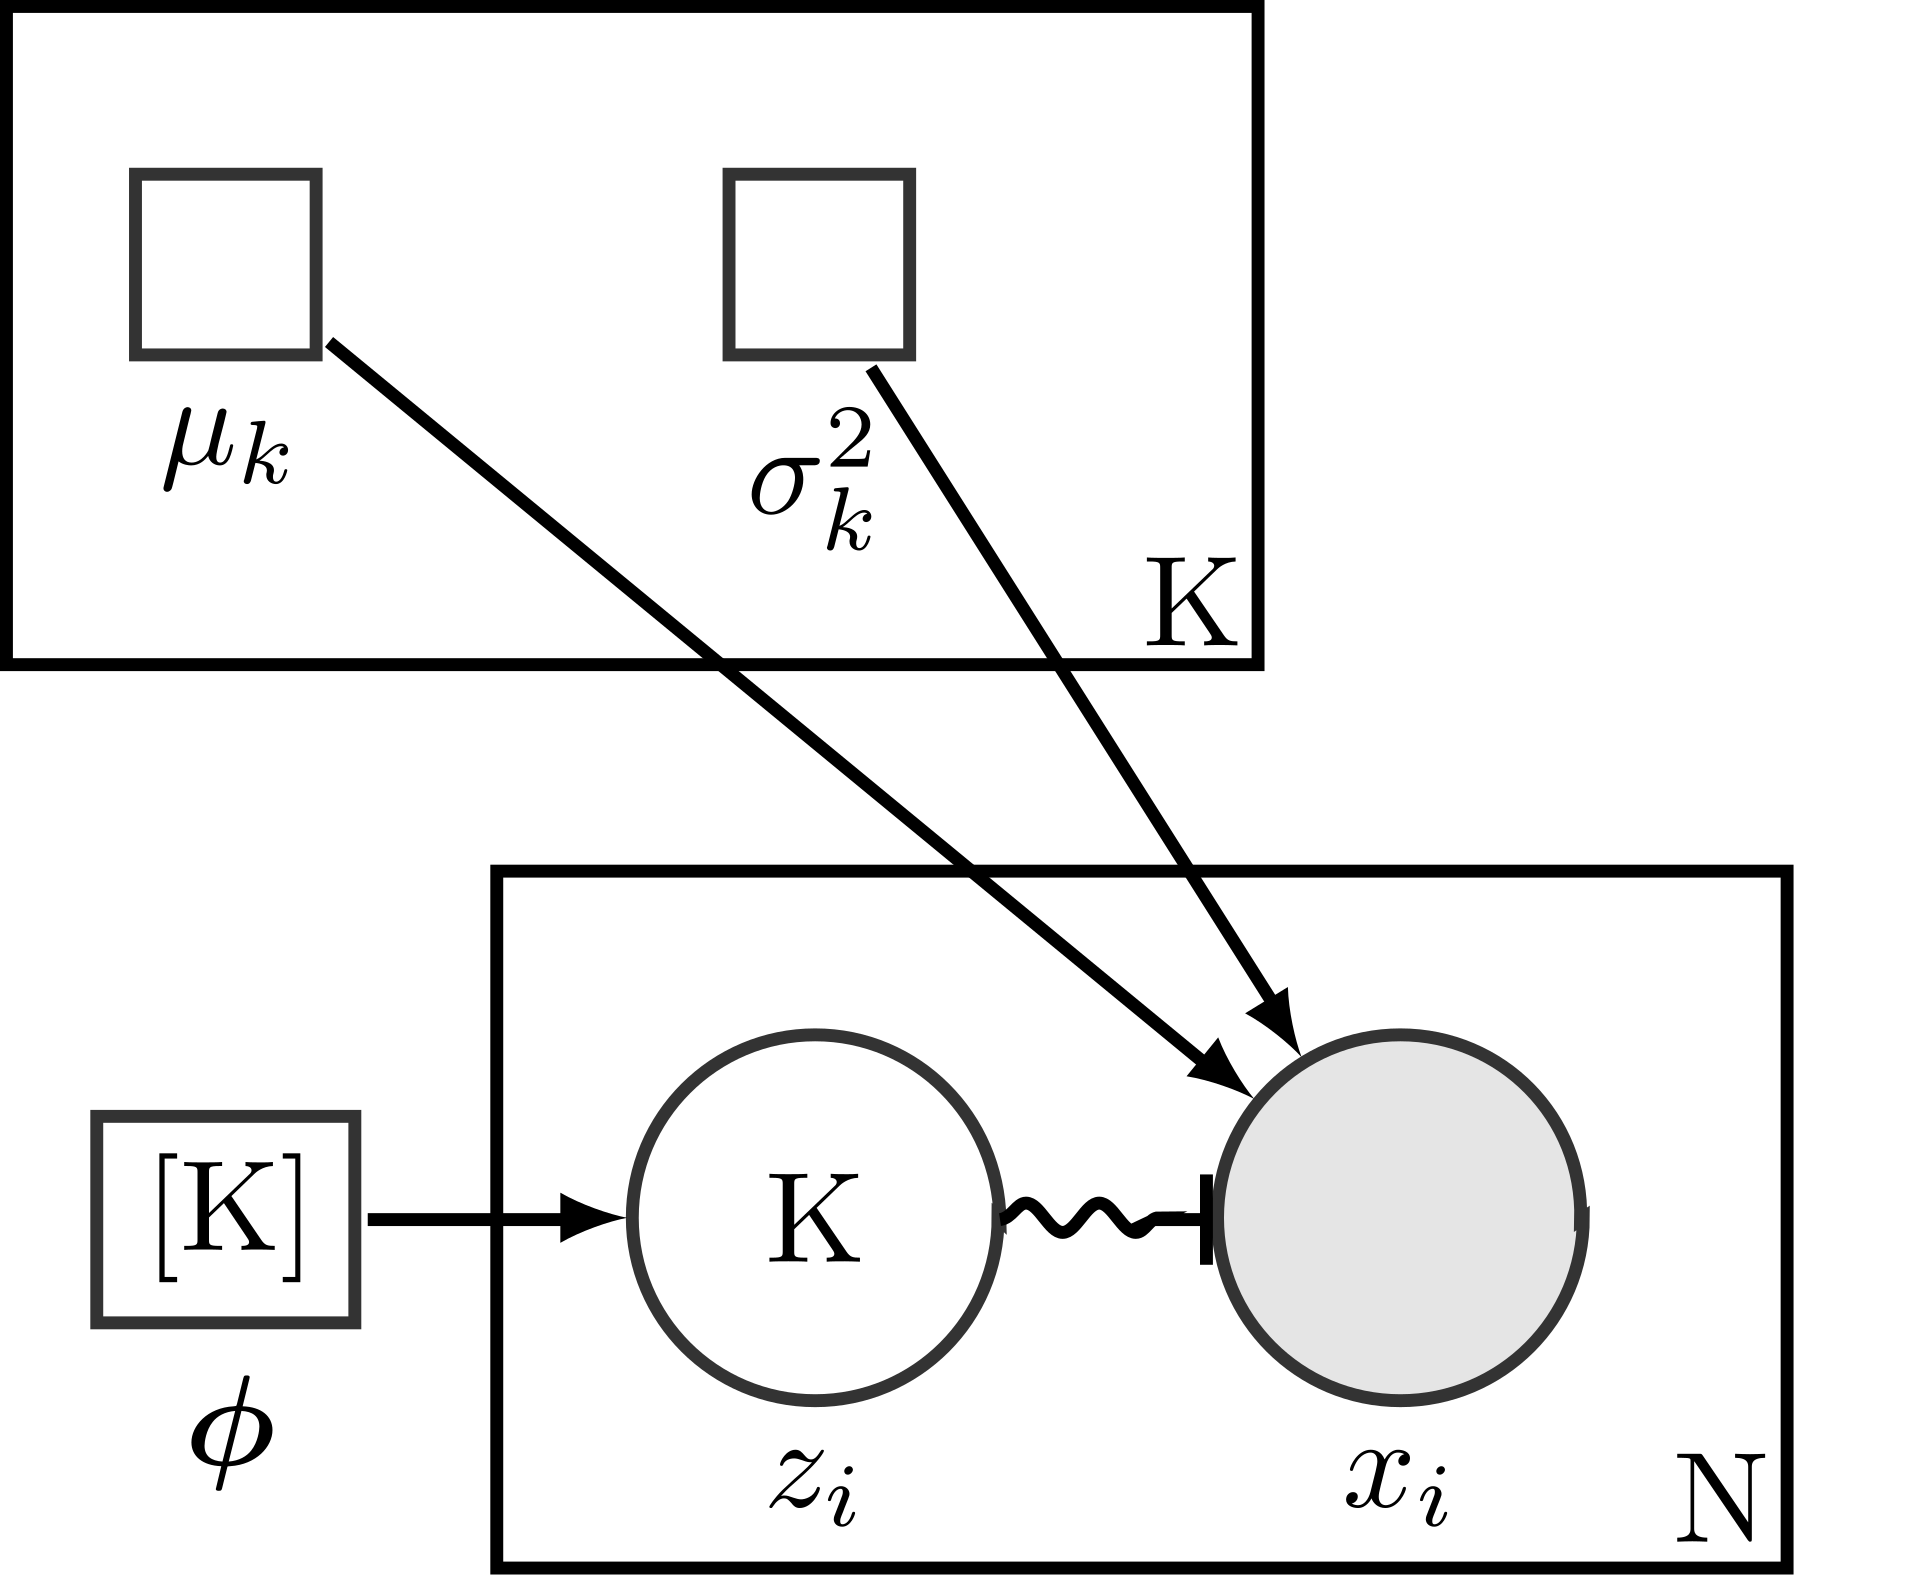
\includegraphics[width=1\linewidth]{images/ComE/GMM.png}
        \caption{Non-Bayesian}
    \end{subfigure}%
    \begin{subfigure}[b]{.5\linewidth}
        \centering
        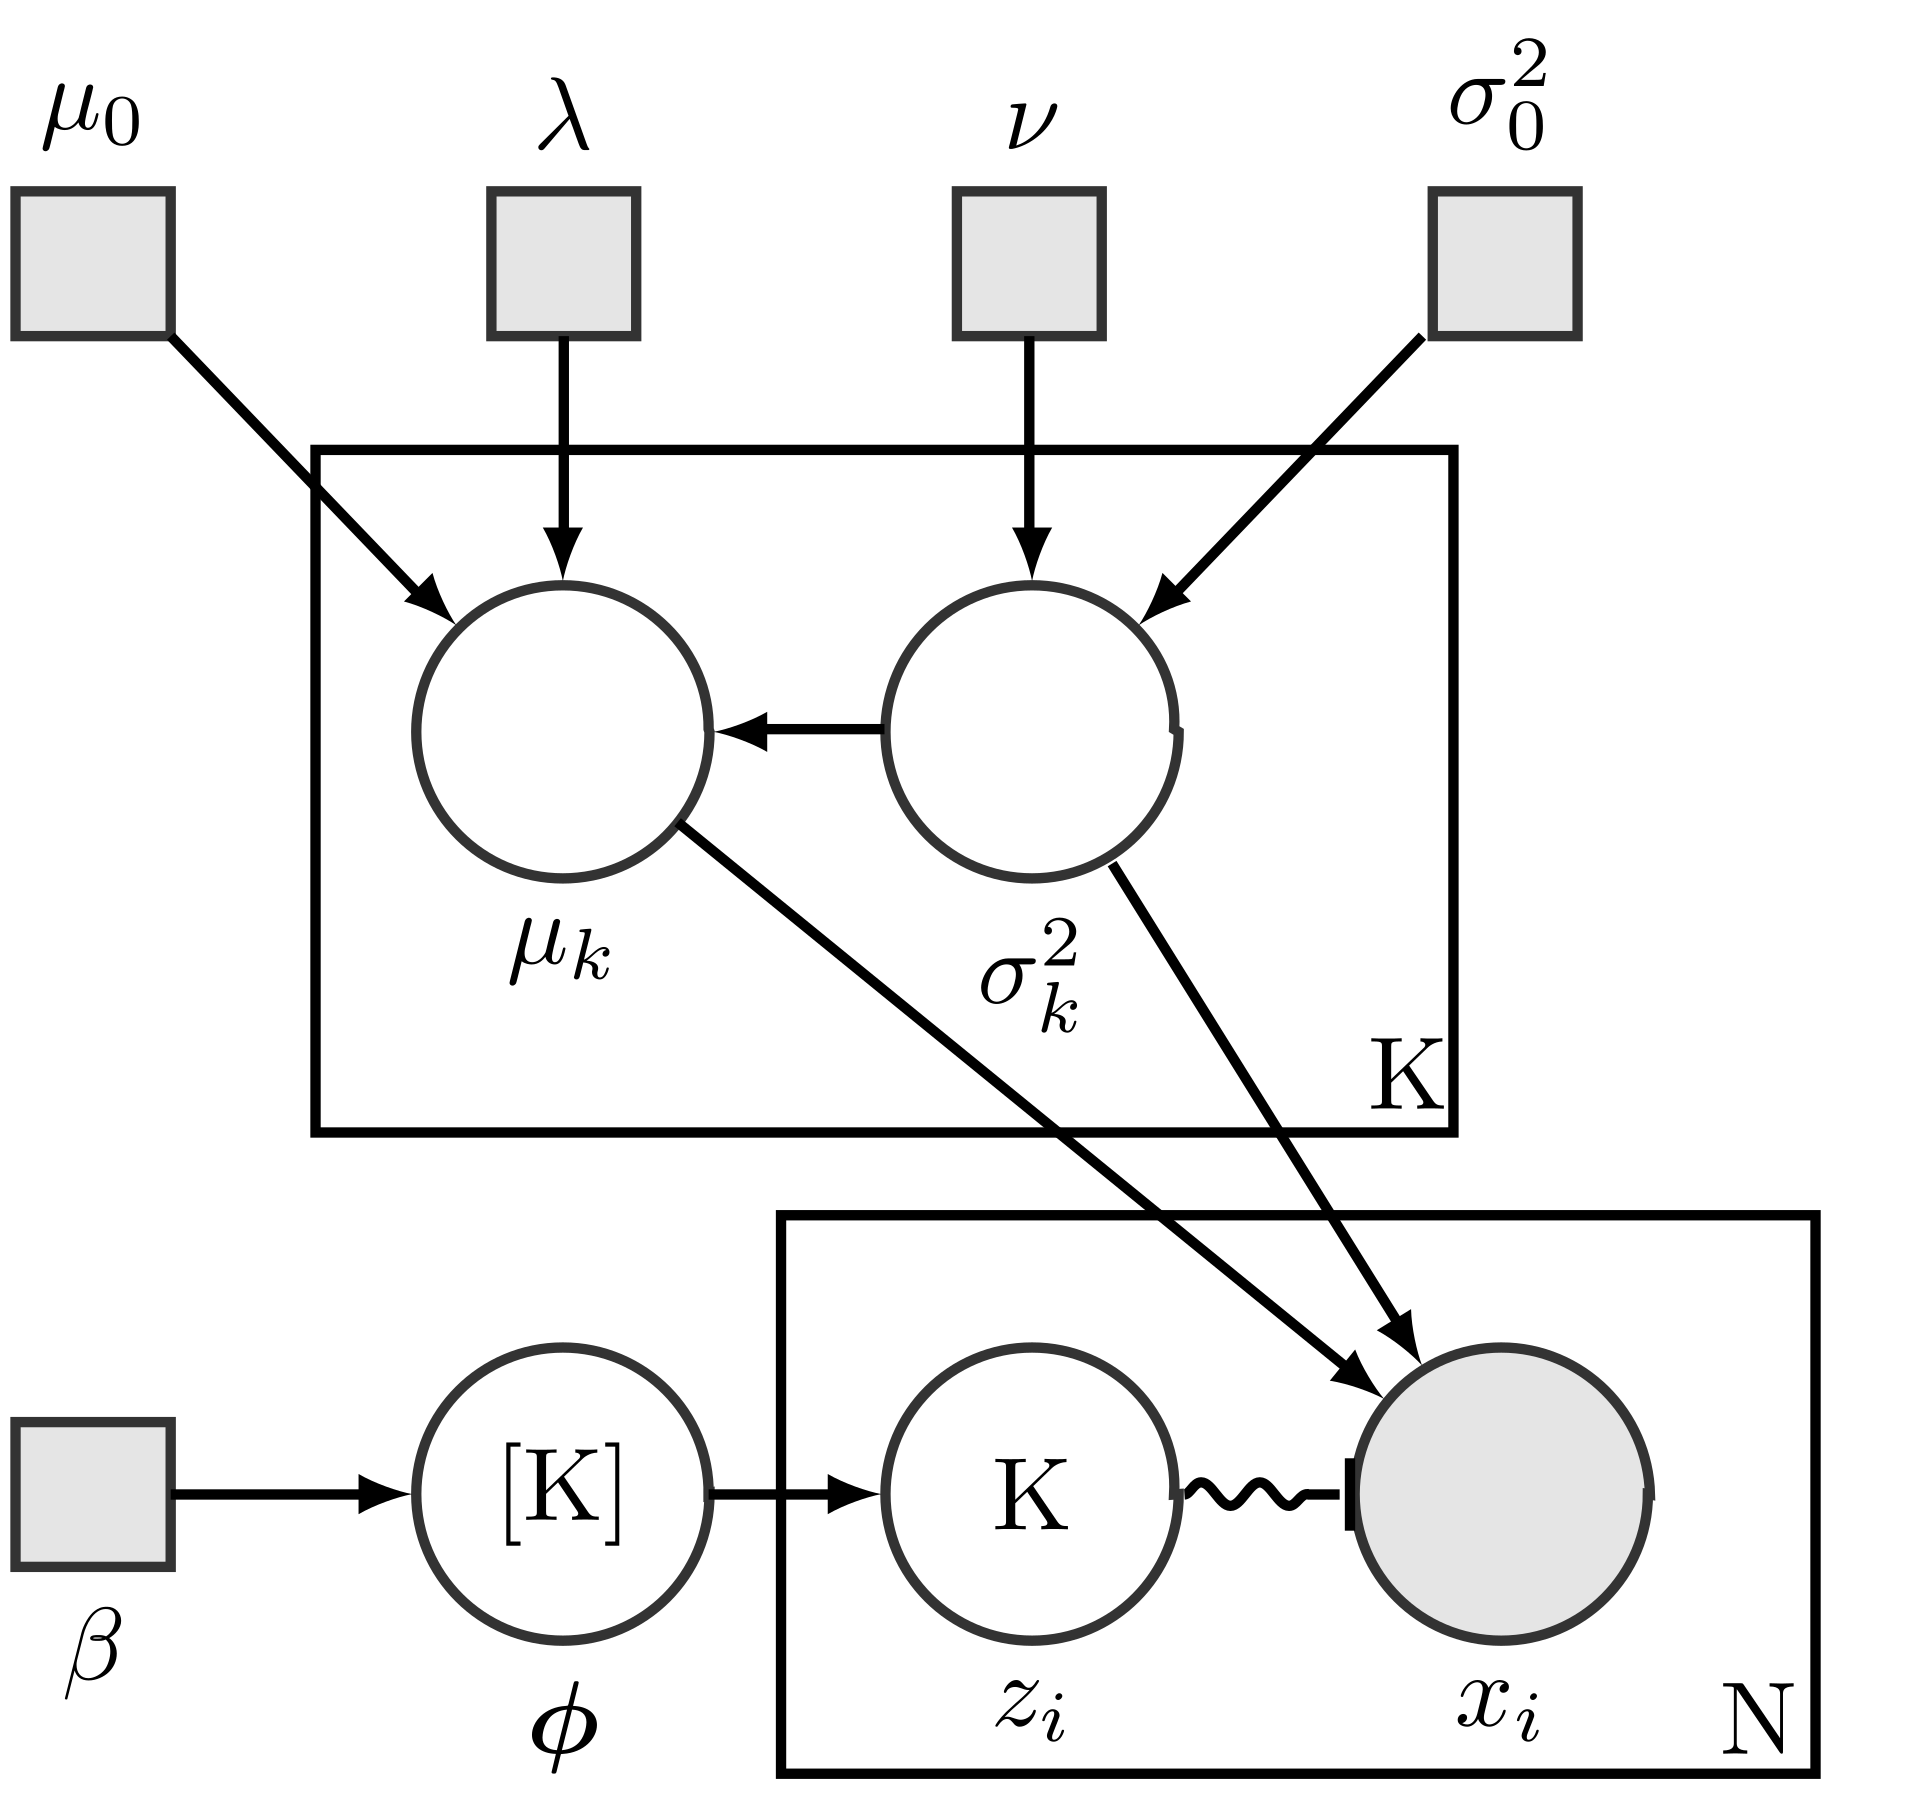
\includegraphics[width=1\linewidth]{images/ComE/BGMM.png}
        \caption{Bayesian}
    \end{subfigure}%
    \caption{Gaussian mixture models in plate notation\protect\footnotemark.}
    \label{fig:GMM_vs_BGMM_plates}
\end{figure}
\footnotetext{By Benwing - Created using LaTeX, TikZ, CC BY 3.0, \url{https://commons.wikimedia.org/w/index.php?curid=18934624}}

Figure \ref{fig:GMM_vs_BGMM_plates} compares a non-Bayesian and a Bayesian GMM side-by-side in plate notation: Squares indicate fixed parameters and circles indicate random variables.

The Bayesian Gaussian mixture model assumes all parameters of the Gaussian mixture model (number of communities $K$, means $\mu_k$, and covariances $\sigma_k$) are themselves generated by some distribution. This is represented in the plate diagrams in Figure \ref{fig:GMM_vs_BGMM_plates}.

A Bayesian Gaussian mixture model (BGMM) with variational inference (VI) offers a solution to the issue of introducing the number of communities $K$ as a fixed parameter, by taking advantage of Bayesian methods.

A BGMM with VI tends to utilize some components heavily while eliminating other components, if the provided dataset suggests so, by applying a tradeoff parameter. Therefore, the parameter $K$ represents a maximum of communities and not the final number of communities like for GMMs.

\subsection{Algorithm ComE BGMM+VI}
\label{sec:ComE_BGMM_alg}

The algorithm can stay mostly unchanged to the algorithm sketched out in Section \ref{sec:ComE_alg}. Only steps 3 and 4 need to be adjusted to handle community detection and embedding and node embeddings using a Bayesian Gaussian mixture model (BGMM) with variational inference (VI) instead of a non-Bayesian Gaussian mixture model (GMM) with expectation-maximization (EM).

A Bayesian Gaussian mixture model, just like a non-Bayesian Gaussian mixture model, produces mixed community membership $\Pi$, which means $\Psi$, and covariances $\Sigma$ for communities based on node embeddings $\Phi$. Therefore, the inputs and outputs of step 3 stay the same.

In their \citeyear{ComE+} paper \textit{Embedding Both Finite and Infinite Communities on Graphs}, \citeauthor{ComE+} present their version of ComE with an infinite Bayesian-approach to community detection and embedding. As of the time of writing of this paper, no source code for ComE+ was published. While ComE+ and ComE BGMM+VI both take a Bayesian approach to community embedding, ComE+ redefined the optimization function for higher-order proximity based on the Bayesian Gaussian mixture model, while ComE BGMM+VI simply uses a BGMM for community embedding and detection and leaves the node embedding step unchanged.

The implementation of ComE BGMM+VI\footnote{ComE BGMM+VI is published at \url{https://github.com/abegehr/ComE_BGMM} \cite{ComE_BGMM_GH}.} presented and used in this paper, utilizes sklearn's implementation of the Bayesian Gaussian mixture model and variational inference references at \textit{sklearn.mixture.BayesianGaussianMixture}.\cite{scikit-learn, sklearn_api}

\subsection{Hyperparameters BGMM}
\label{ComE_BGMM_params}

Switching from the original ComE's GMM to a Bayesian GMM, will require one additional parameter: the BGMM's weight concentration prior, or simply concentration.

The BGMM's concentration is a trade-off parameter that directly influences the number of components utilized for community embedding. A higher concentration parameter leads to more components active. A lower concentration parameter leads to fewer components active.

ComE with BGMM and VI has the same hyperparameters as ComE with GMM and EM, as presented in Section \ref{sec:ComE_params}, and in addition also the following:

\begin{table}[H]
    \centering
    \caption{Hyperparameter added to ComE for supporting a BGMM for community embedding \cite{ComE_BGMM_GH}.}
    \label{table:params_ComE_BGMM}
    \begin{tabularx}{\linewidth}{ l | c | X }
        parameter                    & notation & description                               \\
        \hline
        \hline
        weight\_concentration\_prior & $\Gamma$ & Bayesian GMM's weight concentration prior \\
    \end{tabularx}
\end{table}

\section{Visual Example}
\label{ch:come_visual}

In this section community embeddings based on a standard Gaussian mixture model with expectation-maximization (GMM+EM) and community embeddings based on a Bayesian Gaussian mixture model with variational inference (BGMM+VI) are compared visually. Two-dimensional visualizations are computed on a small graph-dataset using multiple values for the hyperparameter number of communities $K$ to show the advantage of BGMM+VI over GMM+EM under specific conditions.

\subsection{Karate Club Dataset}
\label{sec:karate_club}

\textit{Zachary’s Karate Club graph} is a popular graph dataset for visualizing graph algorithms, due to its small size \cite{KarateClubDS}.

The data was collected from a university karate club by \citeauthor{Zachary1977AnIF} as part of the \citeyear{Zachary1977AnIF} paper \textit{Zachary’s Karate Club graph}. The small Karate Club graph consists of 34 nodes, each representing one person as part of the karate club. The presence of an edge represents a social tie among two members of the group. The absence of an edge represents no social tie among the two members of the group. Edges are bidirectional. \textit{Zachary’s Karate Club graph} provided a binary version (ZACHE) and a weighted version (ZACHC) of the graph. We will consider the binary version of the karate club graph.

The following hyperparameters are used for computing both ComE with GMM and BGMM results:

\begin{table}[H]
    \centering
    \caption{Hyperparameters used for the Karate Club dataset.}
    \label{table:params_KCvisual}
    \begin{tabular}{ l | c | r }
        parameter                    & notation & value        \\
        \hline
        \hline
        number\_walks                & $\gamma$ & $10$         \\
        \hline
        walk\_length                 & $\ell$   & $80$         \\
        \hline
        representation\_size         & $D$      & $2$          \\
        \hline
        num\_workers                 & \empty   & $10$         \\
        \hline
        num\_iter                    & \empty   & $1$          \\
        \hline
        reg\_covar                   & \empty   & $0.00001$    \\
        \hline
        batch\_size                  & \empty   & $50$         \\
        \hline
        window\_size                 & $\zeta$  & $10$         \\
        \hline
        negative                     & $m$      & $5$          \\
        \hline
        lr                           & \empty   & $0.025$      \\
        \hline
        alpha                        & $\alpha$ & $0.1$        \\
        \hline
        beta                         & $\beta$  & $0.1$        \\
        \hline
        down\_sampling               & \empty   & $0.0$        \\
        \hline
        communities                  & $K$      & $[2,3,4,15]$ \\
        \hline
        weight\_concentration\_prior & $\Gamma$ & $10^{-5}$    \\
    \end{tabular}
\end{table}

See Table \ref{table:params_ComE} for a descriptions of the hyperparameters.

For each $K \in [2,3,4,15]$ embeddings based on ComE with GMM and ComE with BGMM are computed. Each combination of a $K$ and choice of a mixture model for community detection and embedding, three charts are obtained:

\begin{enumerate}
    \item Graph: nodes positioned using the Fruchterman-Reingold force-directed (spring) algorithm and colored by community assignment.
    \item Embeddings: obtained node and community embeddings. Ellipses represent communities and the underlying Gaussian component. Points colored by the community assignment represent node embeddings.
    \item Weights: bar chart of weight for each community.
\end{enumerate}

\subsection{K=2}

\visresults{GMM}{2}
\visresults{BGMM}{2}

Figure \ref{fig:resultsGMM2} and Figure \ref{fig:resultsBGMM2}.
Two is the intended number of communities. Setting $K=2$ leads to similar results for both using a GMM and a BGMM for community detection and embedding. Although the labels are inverted, and the separation between both community assignments is slightly different, the general community assignment and structure are the same.

\subsection{K=3}

\visresults{GMM}{3}
\visresults{BGMM}{3}

Figure \ref{fig:resultsGMM3} and Figure \ref{fig:resultsBGMM3}.
Choosing $K=3$ leads to worse results when using a GMM in comparison to the BGMM. The GMM utilizes the three components, while the BGMM drops the unnecessary third component and utilizes only the two necessary components.

\subsection{K=4}

\visresults{GMM}{4}
\visresults{BGMM}{4}

Figure \ref{fig:resultsGMM4} and Figure \ref{fig:resultsBGMM4}.
With $K=4$, the quality of embeddings based on the GMM further declines. The GMM utilizes all four communities. The result obtained by the BGMM also declines for this example, but wins over the GMM. The BGMM utilizes three communities.

\subsection{K=15}

%\visresults{GMM}{15}
%\visresults{BGMM}{15}

Figure \ref{fig:resultsGMM15} and Figure \ref{fig:resultsBGMM15}.
Providing $K=15$ at initialization further underlines the potential advantage of BGMM over GMM. The GMM utilizes all 15 communities. It is clear that in this dataset of 34 nodes, no 15 communities are necessary for proper representation. The BGMM achieves a visually comparable quality to results at $K=2$ and $K=3$ by only utilizing 2 of the maximum 15 communities for representation.

\subsection{Summary}

As hypothesized, the community embedding algorithm ComE underperforms when the hyperparameter number of communities $K$ is unknown. A Bayesian approach with variational inference similar to ComE+ is proposed to use the tradeoff parameter weight concentration before dropping unused communities if $K$ is chosen too high.

The small Karate Club dataset, consisting only of 34 nodes, is used to test the hypothesis through a visual comparison experiment. The Karate Club graph is embedded into two-dimensional Euclidean space with ComE and ComE BGMM+VI for multiple values for the hyperparameter number of communities $K = [2, 3, 4, 15]$. The hypothesized advantage of BGMM over GMM for unknown numbers of communities $K$ when embedding with ComE becomes clear. Even with $K=15$, ComE BGMM+VI identifies the $2$ communities, while the non-Bayesian ComE utilizes all $15$ communities.


\section{Quantitative Evaluation}
\label{ch:come_eval}

In their original \citeyear{ComE} paper \textit{Learning Community Embedding with Community Detection and Node Embedding on Graphs}, \citeauthor{ComE} identify three evaluation tasks for experimentation: graph visualization, community detection and node classification \cite{ComE}. Community detection and node classification can objectively be quantitatively evaluated, while graph visualization is subjectively evaluated.

In this section, community embeddings based on a non-Bayesian Gaussian Mixture Model with Expectation-maximization (GMM+EM), as presented with the ComE algorithm, and community embeddings based on a Bayesian Gaussian Mixture Model with Variational Inference (BGMM+VI), similar to the ComE+ algorithm, are evaluated quantitatively over multiple values for the number of communities $K$ hyperparameter.

\section{DBLP Dataset}

To evaluate ComE GMM+EM and ComE BGMM+VI on the tasks graph visualization, community detection, and node classification, the DBLP dataset is considered:

\begin{table}[H]
    \centering
    \caption{Dataset used for quantitative evaluation.}
    \label{table:evaluation_datasets}
    \begin{tabular}{ c || c | c | c | c }
        \thead{graph                                                                            \\$G=(V, E)$} & \thead{\#(node)\\$\abs{V}$} & \thead{\#(edge)\\$\abs{E}$} & \thead{\#(class)\\$K$} & \thead{\#(label)/node} \\
        \hline
        \hline
        \makecell{DBLP} & \makecell{13,184} & \makecell{48,018} & \makecell{5} & \makecell{$1$} \\
    \end{tabular}
\end{table}

\subsection{Hyperparameters}
\label{sec:come_eval_hyper-params}

For comparability, the same hyperparameters are used for ComE GMM+EM and for the proposed ComE BGMM+VI, with the addition of the weight concentration prior hyperparameter for ComE BGMM+VI. The following hyperparameters were used for evaluating the DBLP dataset:

\begin{table}[H]
    \centering
    \caption{Hyperparameters used for the DBLP dataset. See Table \ref{table:params_ComE} for descriptions of hyperparameters.}
    \label{table:params_DBLP}
    \begin{tabular}{ l | c | r }
        parameter                    & notation & value         \\
        \hline
        \hline
        number\_walks                & $\gamma$ & $10$          \\
        \hline
        walk\_length                 & $\ell$   & $80$          \\
        \hline
        representation\_size         & $D$      & $[128, 2]$    \\
        \hline
        num\_workers                 & \empty   & $10$          \\
        \hline
        num\_iter                    & \empty   & $3$           \\
        \hline
        com\_n\_init                 & \empty   & $10$          \\
        \hline
        reg\_covar                   & \empty   & $0.00001$     \\
        \hline
        batch\_size                  & \empty   & $50$          \\
        \hline
        window\_size                 & $\zeta$  & $10$          \\
        \hline
        negative                     & $m$      & $5$           \\
        \hline
        lr                           & \empty   & $0.025$       \\
        \hline
        alpha                        & $\alpha$ & $0.1$         \\
        \hline
        beta                         & $\beta$  & $0.1$         \\
        \hline
        down\_sampling               & \empty   & $0.0$         \\
        \hline
        communities                  & $K$      & $[2,5,10,20]$ \\
        \hline
        weight\_concentration\_prior & $\Gamma$ & $10^{-5}$     \\
    \end{tabular}
\end{table}

See Table \ref{table:params_ComE} for a descriptions of the hyperparameters.

In addition to varying the hyper-parameter number of communities $K$, the dimensionality of the representation (representation\_size) is varied. The tasks are evaluated for two-dimensional and 128-dimensional embeddings to determine the effect of embedding size on the quality of results.


\subsection{Community Detection}

Community detection references the task of clustering nodes into communities and comparing the detected communities to the true communities as obtained from the true node classifications. The evaluation metrics are conductance and NMI.


\subsubsection{Conductance}

Figure \ref{fig:dblp_conductance} shows the conductance obtained from communities generated with ComE GMM+EM and ComE BGMM+VI on the DBLP graph with two- and 128-dimensional embeddings. Lower conductance is better.

\begin{figure*}[htbp]
    \centering
    \begin{subfigure}{.5\textwidth}
        \centering
        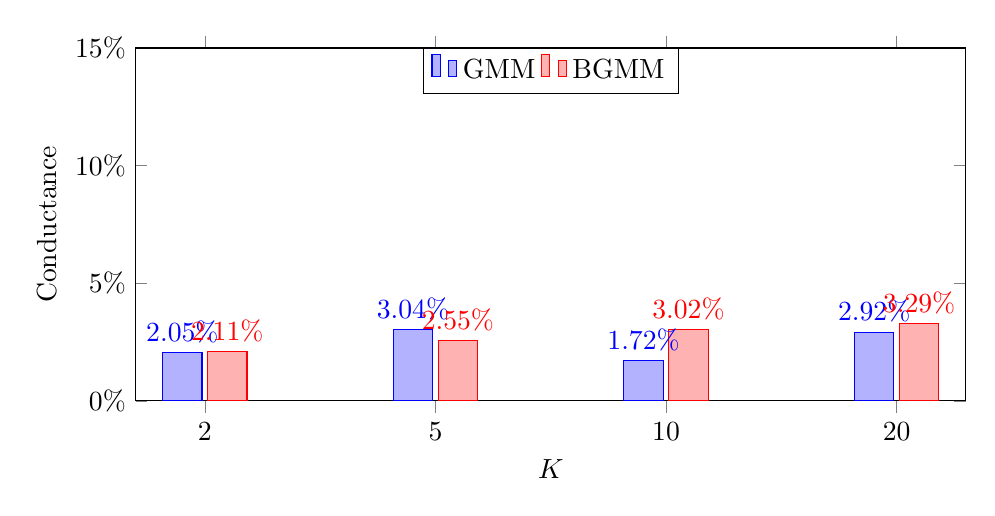
\begin{tikzpicture}
            \pgfplotstableread[row sep=\\,col sep=&]{
                K	& GMM					& BGMM					\\
                2	& 0.02054029917392275	& 0.021070234113712373	\\
                5	& 0.030399077942659558	& 0.02551070276610302	\\
                10	& 0.01722986509950581	& 0.030197444831591175					\\
                20	& 0.029249335242380856	& 0.03289726818006926	\\
            }\mydata
            \begin{axis}[
                    ybar,
                    bar width=.5cm,
                    width=\linewidth,
                    height=.5\linewidth,
                    legend style={at={(0.5,1)},
                            anchor=north,legend columns=-1},
                    symbolic x coords={2,5,10,20},
                    xtick=data,
                    point meta={y*100},
                    yticklabel= {\pgfmathparse{\tick*100}\pgfmathprintnumber{\pgfmathresult}\%},
                    ymin=0, ymax=0.15,
                    xlabel={$K$},
                    ylabel={Conductance},
                    nodes near coords={\pgfmathprintnumber\pgfplotspointmeta\%},
                    nodes near coords align={vertical},
                ]
                \addplot table[x=K,y=GMM]{\mydata};
                \addplot table[x=K,y=BGMM]{\mydata};
                \legend{GMM, BGMM}
            \end{axis}
        \end{tikzpicture}
        \caption{two-dimensional embeddings.}
        \label{fig:dblp_conductance_d2}
    \end{subfigure}%
    %
    \begin{subfigure}{.5\textwidth}
        \centering
        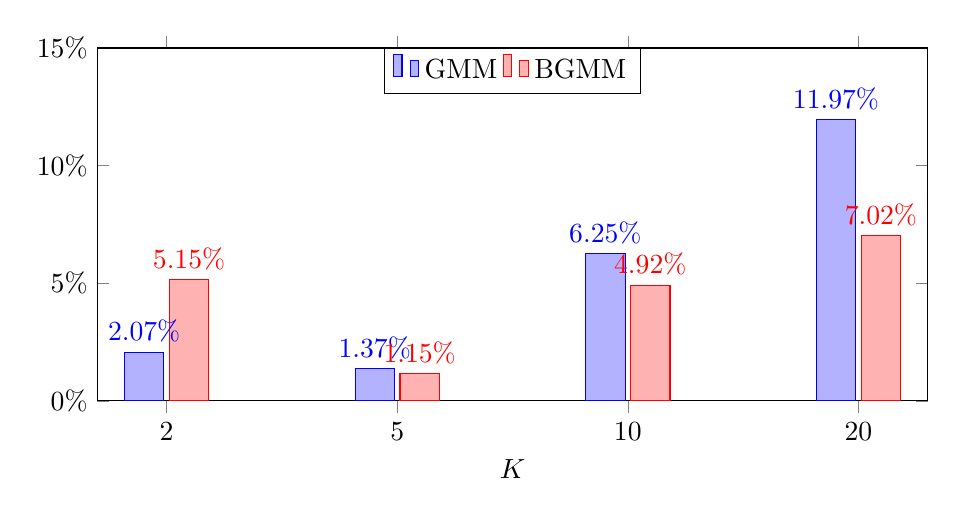
\begin{tikzpicture}
            \pgfplotstableread[row sep=\\,col sep=&]{
                K	& GMM					& BGMM					\\
                2	& 0.02072897576868255	& 0.05153027478804642	\\
                5	& 0.013701852396354014	& 0.011492883939736796	\\
                10	& 0.06247833021288399	& 0.04919872794163497					\\
                20	& 0.11969825263644061	& 0.07018888966334426 \\
            }\mydata
            \begin{axis}[
                    ybar,
                    bar width=.5cm,
                    width=\linewidth,
                    height=.5\linewidth,
                    legend style={at={(0.5,1)},
                            anchor=north,legend columns=-1},
                    symbolic x coords={2,5,10,20},
                    xtick=data,
                    point meta={y*100},
                    yticklabel= {\pgfmathparse{\tick*100}\pgfmathprintnumber{\pgfmathresult}\%},
                    ymin=0, ymax=0.15,
                    xlabel={$K$},
                    nodes near coords={\pgfmathprintnumber\pgfplotspointmeta\%},
                    nodes near coords align={vertical},
                ]
                \addplot table[x=K,y=GMM]{\mydata};
                \addplot table[x=K,y=BGMM]{\mydata};
                \legend{GMM, BGMM}
            \end{axis}
        \end{tikzpicture}
        \caption{128-dimensional embeddings.}
        \label{fig:dblp_conductance_d128}
    \end{subfigure}

    \caption{Conductance on DBLP dataset. Lower conductance is better.}
    \label{fig:dblp_conductance}
\end{figure*}

As was expected, the conductance achieved with the true hyperparameter number of communities $K=5$ is very similar for GMM and BGMM. The conductance achieved for $K=2$ is similar for two-dimensional embeddings and higher for BGMM for 128-dimensional embeddings.

The conductances for $K=10$ and $K=20$ are different depending on the dimensionality of the embedding. For a large representation size of 128 dimensions (see Figure \ref{fig:dblp_conductance_d128}), the conductance for the tested values for $K$ where $K>5$ increases in variability and decreases in overall quality in comparison to the smaller representation size of 2 dimensions (see Figure \ref{fig:dblp_conductance_d2}), where the conductance stays mostly the same with $K=10$ and $K=20$.

Although ComE BGMM+VI produces better conductance than ComE GMM+EM for $K>5$, a clear advantage of BGMM over GMM for community embeddings can not be identified from this experiment alone.

\subsubsection{Normalized Mutual Information}
\label{sec:eval_nmi}

Figure \ref{fig:dblp_nmi} shows the NMIs obtained from communities generated by ComE GMM+EM and ComE BGMM+VI with two- and 128-dimensional embeddings on the DBLP graph. Higher NMI is better.

\begin{figure*}[htbp]
    \centering
    \begin{subfigure}{.5\textwidth}
        \centering
        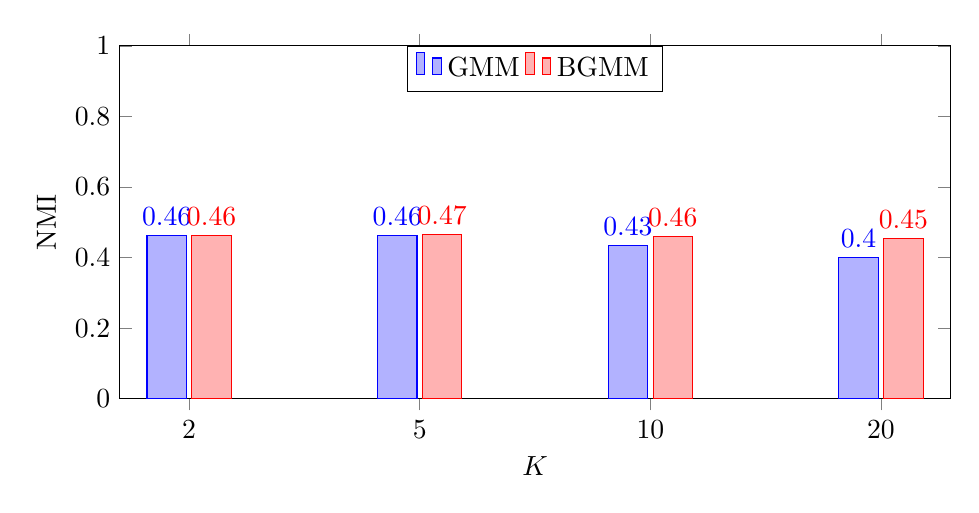
\begin{tikzpicture}
            \pgfplotstableread[row sep=\\,col sep=&]{
                K	& GMM					& BGMM					\\
                2	& 0.4636647057169119	& 0.4623820822063423	\\
                5	& 0.46257130393293455		& 0.46502447614120096		\\
                10	& 0.43349289423082416		& 0.46005304584573076		\\
                20	& 0.3999601374635516	& 0.45371067853180896	\\
            }\mydata
            \begin{axis}[
                    ybar,
                    bar width=.5cm,
                    width=\linewidth,
                    height=.5\linewidth,
                    legend style={at={(0.5,1)},
                            anchor=north,legend columns=-1},
                    symbolic x coords={2,5,10,20},
                    xtick=data,
                    nodes near coords,
                    nodes near coords align={vertical},
                    ymin=0,ymax=1,
                    xlabel={$K$},
                    ylabel={NMI},
                ]
                \addplot table[x=K,y=GMM]{\mydata};
                \addplot table[x=K,y=BGMM]{\mydata};
                \legend{GMM, BGMM}
            \end{axis}
        \end{tikzpicture}
        \caption{two-dimensional embeddings.}
        \label{fig:dblp_nmi_d2}
    \end{subfigure}%
    %
    \begin{subfigure}{.5\textwidth}
        \centering
        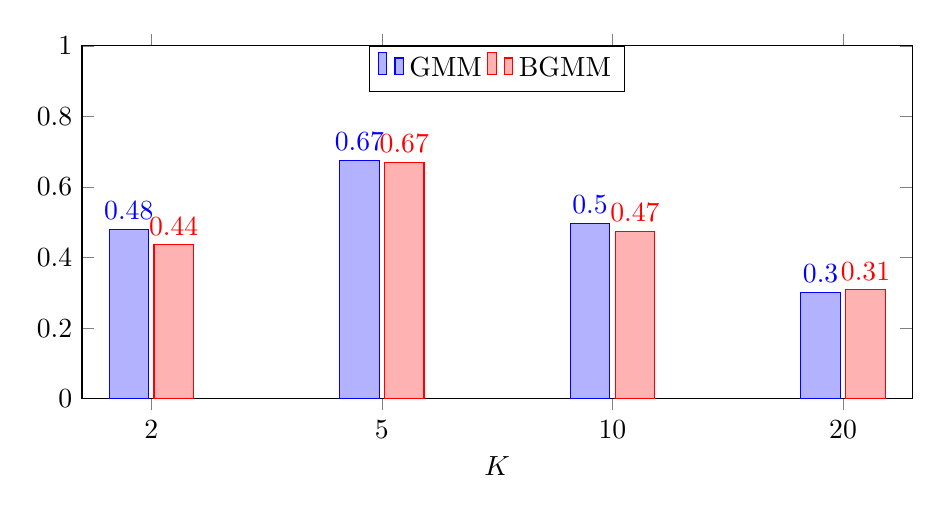
\begin{tikzpicture}
            \pgfplotstableread[row sep=\\,col sep=&]{
                K	& GMM					& BGMM					\\
                2	& 0.4802479401582417	& 0.43575239496704926	\\
                5	& 0.6746848015894669		& 0.668553614850714		\\
                10	& 0.4963225850192131		& 0.47369605057376785		\\
                20	& 0.3018911505699723	& 0.30816578800908423	\\
            }\mydata
            \begin{axis}[
                    ybar,
                    bar width=.5cm,
                    width=\linewidth,
                    height=.5\linewidth,
                    legend style={at={(0.5,1)},
                            anchor=north,legend columns=-1},
                    symbolic x coords={2,5,10,20},
                    xtick=data,
                    nodes near coords,
                    nodes near coords align={vertical},
                    ymin=0,ymax=1,
                    xlabel={$K$},
                ]
                \addplot table[x=K,y=GMM]{\mydata};
                \addplot table[x=K,y=BGMM]{\mydata};
                \legend{GMM, BGMM}
            \end{axis}
        \end{tikzpicture}
        \caption{128-dimensional embeddings.}
        \label{fig:dblp_nmi_d128}
    \end{subfigure}

    \caption{NMI on DBLP dataset. Higher NMI is better.}
    \label{fig:dblp_nmi}
\end{figure*}

ComE GMM+EM and ComE BGMM+VI perform very similar for the true hyperparameter number of communities $K=5$ over both two-dimensional and 128-dimensional embeddings, as was to be expected. The controlling experiment $K=2$ produces similar results for GMM and BGMM as well for both two- and 128-dimensional embeddings.

ComE GMM+EM achieves an NMI of $0.675$ and ComE BGMM+VI achieves an NMI of $0.669$ for the 128-dimensional embedding.
\citeauthor{ComE} state an NMI of over $0.7$ for the ComE algorithm \cite{ComE}. It is not clearly stated how many iterations are run specifically on DBLP in the original ComE paper, but it is stated that ComE converges within two or three iterations.\cite{ComE} In this experiment three iterations were applied, as stated in Section \ref{sec:come_eval_hyper-params}.

With two-dimensional embeddings, an around $0.2$ units smaller NMI is achieved for $K=K^*=5$ than for the 128-dimensional embedding. It seems that the two-dimensional embedding is not capable to capture the complexity of the graph as well as the 128-dimensional embedding.

The advantage of a smaller embedding becomes clearer for larger values of $K>K^*$. For $K=20$ the NMI for the 128-dimensional embedding is around $0.3$, while the BGMM two-dimensional embedding manages to hold at $0.45$.

It seems that for higher $K>5$, ComE BGMM+VI can maintain higher NMI values for the two-dimensional embedding, while for the 128-dimensional embeddings, ComE BGMM+VI is not able to maintain the NMI score. Section \ref{sec:eval_DBLP_result_k} explores the different behavior of ComE BGMM+VI on low- and higher-dimensional embeddings further in comparison to ComE GMM+EM.


\subsection{Number of Communities and Dimensionality}
\label{sec:eval_DBLP_result_k}

To understand why ComE BGMM+VI is able to maintain an NMI score for larger values of $K$ for the two-dimensional embedding, but not for the 128-dimensional embedding, the weights of the components for $K=20$ is presented:

\begin{figure}[H]
    \centering
    % K=5
    \begin{subfigure}[b]{.5\linewidth}
        \centering
        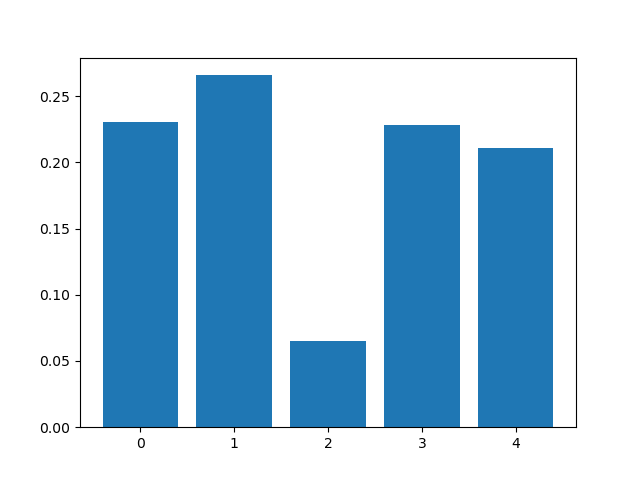
\includegraphics[width=1\linewidth]{images/eval/weights_BGMM_d2_k5.png}
        \caption{D=2, K=5}
        \label{fig:dblp_weights_d2_k5}
    \end{subfigure}%
    %
    \begin{subfigure}[b]{.5\linewidth}
        \centering
        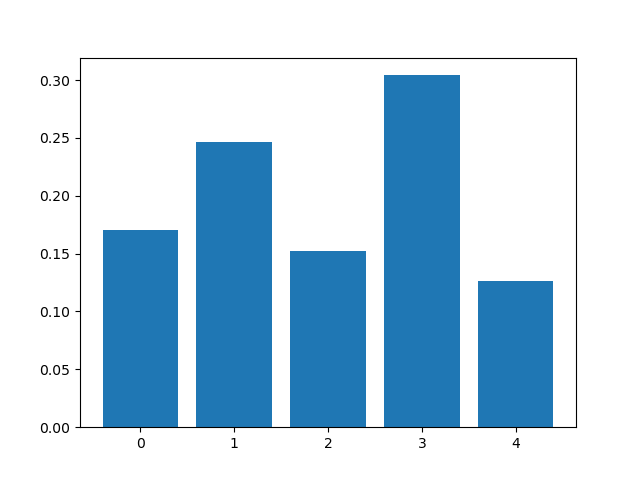
\includegraphics[width=1\linewidth]{images/eval/weights_BGMM_d128_k5.png}
        \caption{D=128, K=5}
        \label{fig:dblp_weights_d128_k5}
    \end{subfigure}
    % K=10
    \begin{subfigure}[b]{.5\linewidth}
        \centering
        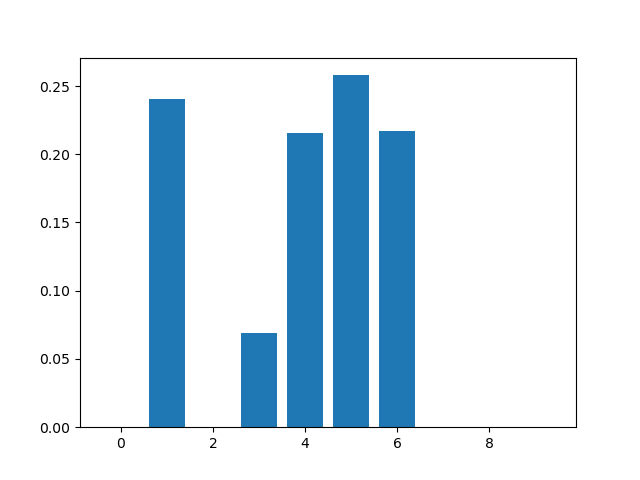
\includegraphics[width=1\linewidth]{images/eval/weights_BGMM_d2_k10.png}
        \caption{D=2, K=10}
        \label{fig:dblp_weights_d2_k10}
    \end{subfigure}%
    %
    \begin{subfigure}[b]{.5\linewidth}
        \centering
        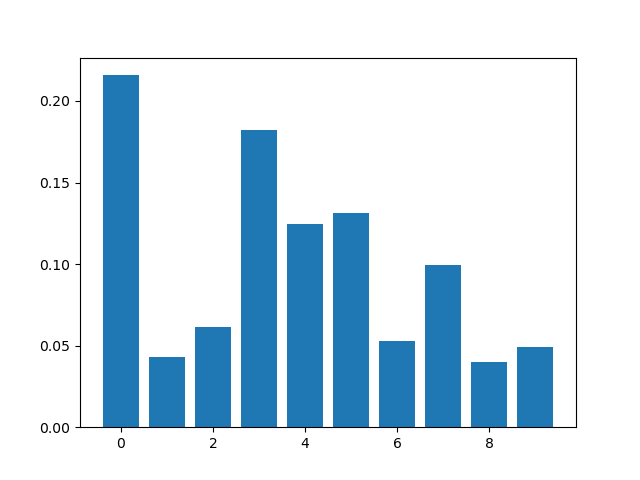
\includegraphics[width=1\linewidth]{images/eval/weights_BGMM_d128_k10.png}
        \caption{D=128, K=10}
        \label{fig:dblp_weights_d128_k10}
    \end{subfigure}
    % K=20
    \begin{subfigure}[b]{.5\linewidth}
        \centering
        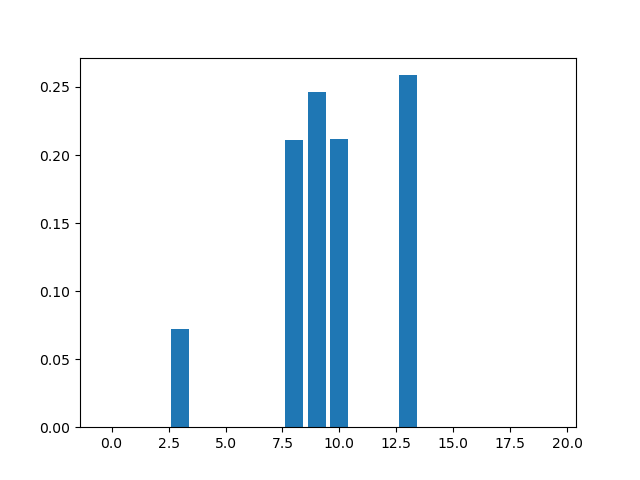
\includegraphics[width=1\linewidth]{images/eval/weights_BGMM_d2_k20.png}
        \caption{D=2, K=20}
        \label{fig:dblp_weights_d2_k20}
    \end{subfigure}%
    %
    \begin{subfigure}[b]{.5\linewidth}
        \centering
        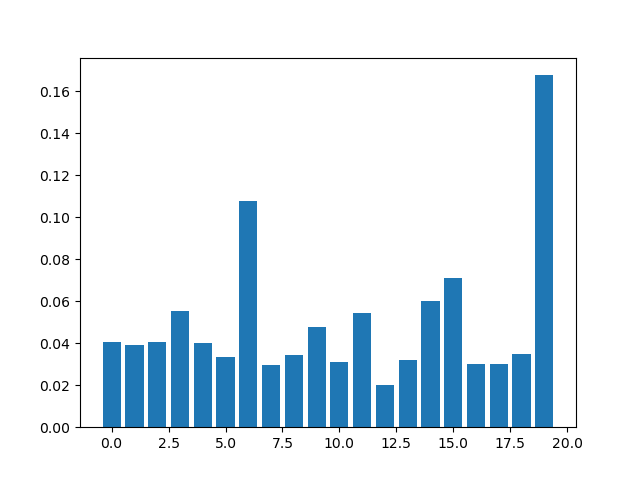
\includegraphics[width=1\linewidth]{images/eval/weights_BGMM_d128_k20.png}
        \caption{D=128, K=20}
        \label{fig:dblp_weights_d128_k20}
    \end{subfigure}

    \caption{Weights of communties generated by ComE BGMM+VI over hyperparameters representation sizes $D=[2, 128]$ and number of communities $K=[5, 10, 20]$.}
    \label{fig:dblp_weights}
\end{figure}

Figure \ref{fig:dblp_weights} shows in subfigures \ref{fig:dblp_weights_d2_k5}, \ref{fig:dblp_weights_d2_k10}, and \ref{fig:dblp_weights_d2_k20}, that ComE BGMM+VI is able to identify $K=5$ communities for the initial hyperparameter settings $K=[5, 10, 20]$ if a two-dimensional embedding is choosen. For the 128-dimensional embeddings in subfigures \ref{fig:dblp_weights_d128_k5}, \ref{fig:dblp_weights_d128_k10}, and \ref{fig:dblp_weights_d128_k20}, ComE BGMM+VI is not able to drop communities to identify the $K=5$ with initial values of $K=[5,10,20]$.

The finding from comparing community weights over the two- and 128-dimensional embedding of ComE BGMM+VI not dropping components for the 128-dimensional embeddings could explain the observation in Section \ref{sec:eval_nmi} of a better NMI for $D=2$ when $K=20$.

It is left for future work to consider different weight concentration priors and further explorations into the ability of BGMM and variational inference to unused drop components dependant of the dimensionality of input space.


\section{Results of Node Classification}

Figure \ref{table:dblp_f1} shows the results of ComE GMM+EM and ComE BGMM+VI on the task node classification compared over multiple values for the hyperparameter number of communities $K$. The evaluation metrics micro- and macro-F1 are used.

First, embeddings are generated from the whole graph. Then, node classification is done by a support vector machine (SVM), which is trained on $90\%$ of the node embeddings and tested on the remaining $10\%$ of node embeddings. The two- or 128-dimensional node embeddings are used as features for the support vector machine.

\begin{figure}[H]
    \centering

    \begin{subfigure}[b]{\linewidth}
        \begin{table}[H]
            \centering
            \begin{tabular}{ l | l | c | c | c | c }
                \hline
                \empty                         & \#(communities) $K$ & 2             & 5             & 10            & 20            \\
                \hline
                \hline
                \multirow{2}{*}{Micro-F1 (\%)} & ComE BGMM+VI        & \textbf{67.1} & 67.2          & 66.2          & \textbf{67.0} \\
                                               & ComE                & 66.9          & \textbf{67.4} & \textbf{66.6} & 66.5          \\
                \hline
                \multirow{2}{*}{Macro-F1 (\%)} & ComE BGMM+VI        & \textbf{50.9} & 49.6          & 48.6          & \textbf{49.6} \\
                                               & ComE                & 50.0          & \textbf{50.0} & \textbf{49.3} & 49.0          \\
                \hline
            \end{tabular}
            \caption{two-dimensional embeddings.}
            \label{table:dblp_f1_d2}
        \end{table}
    \end{subfigure}

    \begin{subfigure}[b]{\linewidth}
        \begin{table}[H]
            \centering
            \begin{tabular}{ l | l | c | c | c | c }
                \hline
                \empty                         & \#(communities) $K$ & 2             & 5             & 10            & 20            \\
                \hline
                \hline
                \multirow{2}{*}{Micro-F1 (\%)} & ComE BGMM+VI        & 92.6          & \textbf{92.6} & \textbf{93.3} & 92.3          \\
                                               & ComE                & 92.6          & 92.5          & 93.2          & \textbf{92.7} \\
                \hline
                \multirow{2}{*}{Macro-F1 (\%)} & ComE BGMM+VI        & \textbf{92.7} & \textbf{92.4} & \textbf{93.0} & 91.9          \\
                                               & ComE                & 92.6          & 92.3          & 92.9          & \textbf{92.7} \\
                \hline
            \end{tabular}
            \caption{128-dimensional embeddings.}
            \label{table:dblp_f1_d128}
        \end{table}
    \end{subfigure}

    \caption{Micro- and Macro-F1 on the DBLP dataset with two- and 128-dimensional embeddings. Higher F1 values are better.}
    \label{table:dblp_f1}
\end{figure}

The Micro- and Macro-F1 scores attained by ComE GMM+EM and ComE BGMM+VI node embeddings through an SVM are very similar. No advantage of one over the other can be determined from the results. The similarity between results for node classification could be due to the specialties of the used DBLP dataset. To gain more clarity, further datasets should be evaluated in future work.


\subsection{Summary}

Although a better conductance was achieved for large $K$ on the 128-dimensional embedding, a clear advantage of ComE BGMM+VI over ComE GMM+EM can not be identified for conductance over one experiment.

For NMI, ComE BGMM+VI seems to perform slightly better than ComE when choosing a two-dimensional embedding instead of a 128-dimensional embedding and a greater initial number of communities that the true number of communities: $K>5$. It is hypothesized that this advantage comes from the ability of BGMM+VI to drop unused components in lower-dimensional space. It appears that BGMM+VI does not drop components as easy in higher-dimensional space.

Examining the weights of components produced by ComE BGMM+VI in two- and 128-dimensional space provides the insight, that ComE BGMM+VI produces the same distributions of 5 components' weights for $K=5$, $K=10$, and $K=20$ in two-dimensional space. In 128-dimensional space, on the other hand, ComE BGMM+VI does not drop components and remains with weight distributions including all the components added at initialization.

In the experiment on the DBLP dataset, no advantage of using ComE BGMM+VI over GMM+EM was identified for node classification by SVM. It is reasonable to note, that node classification with micro- and macro-F1 of over $90\%$ is achieved, with the 128-dimensional embedding, leaving little room for optimization.

A slight advantage of ComE BGMM+VI over ComE GMM+EM for community detection over the DBLP dataset under specific conditions was identified. No advantage for the task of node classification for ComE BGMM+VI over ComE GMM+EM could be identified for the DBLP dataset.

It was identified, that while the BGMM with variational inference can drop unused components when operating in low dimensional space and achieve the same component weight distributions over multiple initial values for $K$, in high dimensional space, the BGMM does not drop components.

\section{Conclusion}

ComE BGMM+VI, an extension of the community embedding algorithm ComE is presented in this paper. ComE BGMM+VI utilizes a Bayesian Gaussian mixture model instead of a non-Bayesian Gaussian mixture model for community embedding and detection. The Bayesian community embedding algorithm ComE BGMM+VI is compared to ComE GMM+EM visually on the Karate Club graph dataset and quantitatively evaluated on community detection and node classification the DBLP dataset.

Visually comparing ComE BGMM+VI to ComE GMM+EM clearly shows the advantage of ComE BGMM+VI over ComE GMM+EM for an unknown number of communities $K$ and a low representation size $D$. ComE BGMM+VI is able to drop unused communities and reduce $K$ to the number of communities present at the resolution captured at the chosen representation size $D$ through the weight concentration prior hyperparameter trade-off parameter.

A slight edge of ComE BGMM+VI over the original ComE as identified for community detection NMI in a low-dimensional embedding for $K$ larger than the true number of communities. More notably, ComE BGMM+VI captures 5 communities in the DBLP dataset at representation size $D=2$ for all tested values for the number of communities $K>5$. The true number of communities in the DBLP dataset is 5. ComE with non-Bayesian Gaussian mixture model is not able to drop communities for $K>5$, as seen in Figure \ref{fig:dblp_weights}.



















%%% Bibliography
\bibliographystyle{IEEEtranN}
\bibliography{literature}

\end{document}
